\documentclass{beamer}

\usepackage{beamerthemesplit}
\usepackage{verbatim}

\usetheme{Pittsburgh}
%\usecolortheme{seagull}
%\usecolortheme{seahorse}
\usecolortheme{beaver}

\usefonttheme{serif}

%\DeclareGraphicsExtensions{.pdf,.png,.jpg}

\newcommand{\snT}{$(S/N)_{\textrm{size}}$}
%\newcommand{\snT}{$\left( \frac{S}{N}\right)_{\textrm{size}}$}
\newcommand{\snflux}{$(S/N)_{\textrm{flux}}$}
%\newcommand{\snflux}{$\left( \frac{S}{N}\right)_{\textrm{flux}}$}

\newcommand{\lensfit}{\texttt{LENSFIT}}
\newcommand{\numba}{\texttt{Numba}}
\newcommand{\python}{\texttt{Python}}
\newcommand{\ngmix}{\texttt{ngmix}}
\newcommand{\shear}{{\bf g}}

\title{Weak Lensing Results from DES}
\author{Erin Sheldon}
\institute{Brookhaven National Laboratory}

% http://texblog.net/latex-archive/plaintex/beamer-footline-frame-number/
% to add the page (frame ) number and not screw up the bottom line
% works for split themes?
\expandafter\def\expandafter\insertshorttitle\expandafter{%
      \insertshorttitle\hfill%
        \insertframenumber\,/\,\inserttotalframenumber}

% suppress navigation bar
\beamertemplatenavigationsymbolsempty

\begin{document}

%\frame{\titlepage}

%\section{Dark Energy}

\frame
{
    \frametitle{Dark Energy}

    \fontsize{9}{0.8\baselineskip}
    \begin{columns}
        \begin{column}{0.5\textwidth}    
            \begin{itemize}
                \item The original story is simple

                \item There are objects whose intrinsic brightness we think we
                    know (type 1a supernovae)

                \item If we know one of these objects is at a given distance we
                    should be able to predict its observed brightness

                \item It turns out this only works if we modify the equations
                    so that the universe is accelerating at late times (long
                    after the big bang, recently) instead of slowing down

                \item Either add a new component, such as a cosmological constant,
                    or modify general relativity

            \end{itemize}
        \end{column}
        \begin{column}{0.5\textwidth}
            \begin{center}
                \includegraphics[width=\textwidth]{riess-distmodulus.pdf}
                \newline
                Riess et al. 2007
            \end{center}
        \end{column}
    \end{columns}
}

\frame
{
    \frametitle{Standard Rulers}

    \fontsize{9}{0.8\baselineskip}
    \begin{columns}
        \begin{column}{0.5\textwidth}    
            \begin{itemize}

                \item The baryon acoustic feature is frozen in when the
                    universe cools enough for baryons and photons to decouple:
                    it is thus a standard ruler

                \item its apparent size at a give distance should be predictable
                    given the observed size in the CMB and a cosmological model.

                \item again, it only works if we modify the equations

            \end{itemize}
        \end{column}
        \begin{column}{0.5\textwidth}
            \begin{center}
                \includegraphics[width=\textwidth]{bao-all.pdf}
                \newline
                Aubourg et al. 2014 (BOSS)
            \end{center}
        \end{column}
    \end{columns}
}

\frame
{
    \frametitle{Simplest Possible Components}

    \begin{itemize}

        \item Add a constant energy density component to the stress-energy:   A
            cosmological constant $\Lambda$ that has equation of
            state  $p=-\rho$.
            
        \item Constant energy density in an expanding universe is unsatisfying,
            but it matches the data well with our current limited precision.

        \item Next level of complexity: arbitrary equation of state.  This is
            poorly constrained with current data.

    \end{itemize}

    \begin{equation}
        p = w \rho
    \end{equation}

    \begin{itemize}
        \item Any accelerating solution for $w$ ($< - 1/3$) violates the strong energy condition.
    \end{itemize}

}



\frame
{
    \frametitle{Gravitational Lensing}

    \begin{itemize}

        \item Light is apparently deflected as it passes massive bodies.

        \item All objects in the universe are lensed.

        \item As with an ordinary lens, the deflection at the detector depends
            on the strength of the lens and the geometry of the
            lens-source-observer system

        \item The geometry depends on dark energy.
            
        \begin{itemize}
            \item We can use this to measure dark matter and dark energy
        \end{itemize}

    \end{itemize}

}

\frame
{
    \frametitle{Lensing Geometry}

    \includegraphics[width=\textwidth]{lens_geometry.pdf}

}

\frame
{
    \frametitle{Example: Lensing Geometry and Dark Energy}

    %\fontsize{9}{0.8\baselineskip}
    \begin{columns}
        \begin{column}{0.5\textwidth}    
            \begin{itemize}

                \item The signal depends on the distance of source behind
                    the lens.


                \item Measure the lensing effect using the same lens and sources
                    at different distances

                \item the mapping beteween distance and observables (redshift) 
                    depends on dark energy

                \item What value of the equation of state $w$ do we need to
                    describe the observations?

            \end{itemize}
        \end{column}
        \begin{column}{0.5\textwidth}
            \includegraphics[width=\textwidth]{scinv-example.pdf}
        \end{column}
    \end{columns}
}


\frame
{
    \frametitle{Lensing Reality}

    \begin{center}
        \includegraphics[width=\textwidth]{shear-illustration.jpg}
        \newline
    \end{center}

}


\frame
{

    \frametitle{Weak Lensing}

    \fontsize{10}{0.8\baselineskip}

    \begin{columns}

        \begin{column}{0.5\textwidth}

            \begin{itemize}

                \item We don't see the deflection directly.

                \item The ``deflection'' can differ across the face of an
                    extended source galaxy, causing distortion.

                \item We say the image is ``sheared'' (a light bundle 
                    is sheared)

                \item For small shears, a circle becomes a pure ellipse.

                \item Shearing produces correlations in the shapes of galaxies across the sky.
                    Shape correlations are closely related to mass density
                    correlations.

            \end{itemize}
        \end{column}
        \begin{column}{0.5\textwidth}
            \includegraphics[width=\textwidth]{shear-illustration-crop.jpg}
            \newline
            \begin{center}
                {\small Note galaxies aren't round!  ``Shape noise''}
            \end{center}
        \end{column}
    \end{columns}
}

\frame
{
    \frametitle{Shear}
    %\fontsize{10}{0.8\baselineskip}

    \begin{columns}
        \begin{column}{0.5\textwidth}
            \begin{itemize}


                \item The correlations in the shear/matter field hold a lot of
                    information about the {\bf Dark Matter} distribution.  The Cold Dark
                    Matter theory predicts these correlations.

                \item Shear depends on the distances to the lens and source. The
                    distance dependence encodes the expansion rate of the universe and
                    thus {\bf Dark Energy}.

                %\item To meet goals of current surveys we want to measure shear to
                %    about 0.4\% accuracy (e.g.  Dark Energy Survey).  LSST about
                %    a factor of five better.

            \end{itemize}
        \end{column}

        \begin{column}{0.5\textwidth}
                \includegraphics[width=\textwidth]{berlind-weinberg-f3.pdf}
                \newline
                Berlind \& Weinberg 2002
                \newline
                Dark Matter Prediction
        \end{column}
    \end{columns}
}


\frame
{
    \frametitle{Lensing Dark Energy State of the Art}

    \begin{center}
        \includegraphics[width=\textwidth]{cfht-wmap.pdf}
        \newline
        Kitching et al. 2015, CFHTLens.  Pure ``Cosmic Shear'' measurement.
    \end{center}

}



\frame
{
    \frametitle{Shear From Galaxy Clusters}

    \begin{center}
        \includegraphics[width=0.8\textwidth]{maxbcg_sample21-22_ngals200_12_jackknife.pdf}
        \newline
        Sheldon et al. 2009.  Sloan Digital Sky Survey Galaxy Clusters
    \end{center}
}



\frame
{
    \frametitle{Galaxy Clusters in the SDSS}
    \fontsize{10}{0.8\baselineskip}

    \begin{columns}
        \begin{column}{0.5\textwidth}
            \begin{itemize}

                \item This technique is well established, and measured with high precision.

                \item In SDSS we used lensing to study the dark matter distribution in
                    and around galaxy clusters.

                \item SDSS is a low redshift survey, no sensitivity to dark energy.

                \item Similar measurements by other surveys (e.g. CFHT, Weighing the Giants)
                    as well as more generic shear measurements (``Cosmic Shear'')

            \end{itemize}
        \end{column}

        \begin{column}{0.5\textwidth}
            \includegraphics[width=\textwidth]{maxbcg_sample21-22_ngals200_12_jackknife.pdf}
            \newline
            Sheldon et al. 2009
        \end{column}
    \end{columns}
}


\frame
{
    \frametitle{Dark Energy Survey (DES)}

    \fontsize{9}{0.8\baselineskip}
    \begin{columns}
        \begin{column}{0.5\textwidth}    
            \begin{itemize}

                \item Imaging survey of 5000 square degrees in the 
                    southern sky (CTIO) through 5 optical filters.  Dept $\sim 24$ in
                    $i$-band.

                \item Study dark energy using weak lensing, galaxy clusters, supernovae
                    and large scale structure (BAO).

                \item First light fall 2012, survey start Aug. 31 2013
                    
                \item Can repeat SDSS cluster measurements with equal S/N at
                    many redshifts: Dark Energy

                \item Next generation:  reduce the errors on $w$ to the percent level.

            \end{itemize}
        \end{column}
        \begin{column}{0.5\textwidth}
            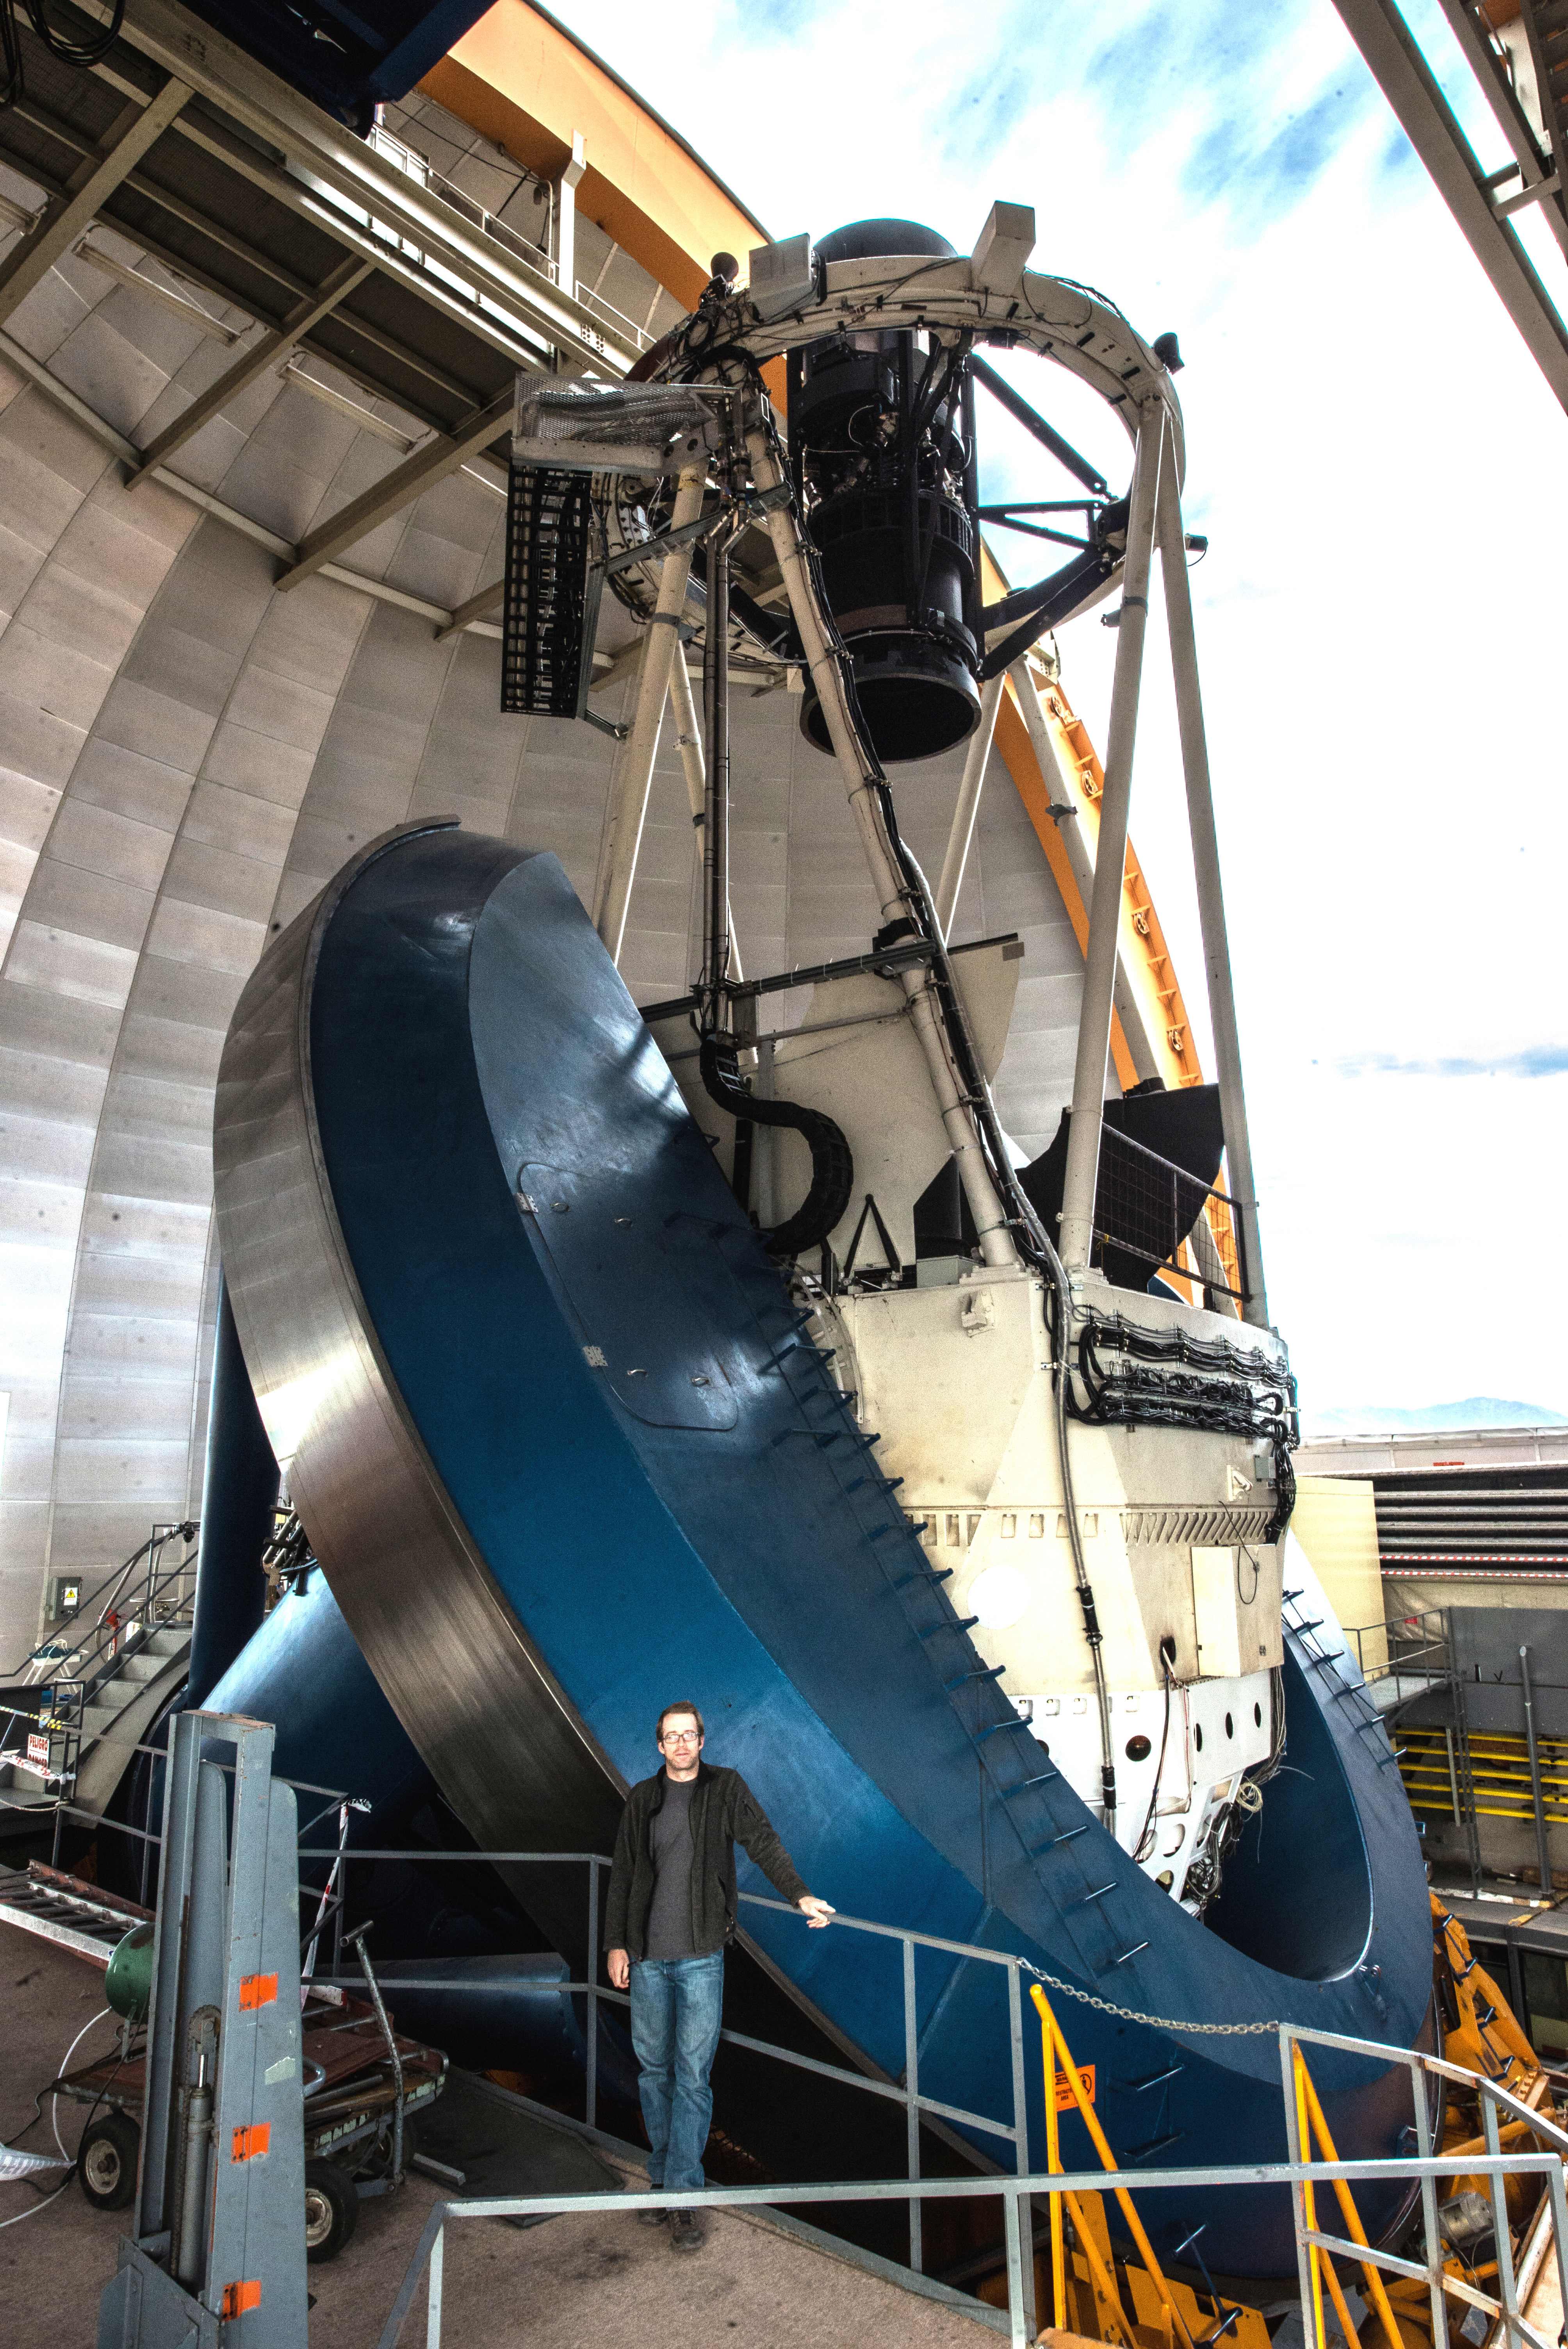
\includegraphics[width=\textwidth]{ctio_blanco_crew_2013Oct-19-contrast.jpg}
        \end{column}
    \end{columns}
}


\frame
{
    \frametitle{What is needed to achieve DES goals}

    %\fontsize{9}{0.8\baselineskip}
    \begin{itemize}

        \item Measure the shears with $\sim$ 0.4\% accuracy

            \begin{itemize}
                \item Develop galaxy shape measurement algorithms
            \end{itemize}

        \item Measure the distances with equal accuracy.

        \begin{itemize}
            \item No spectra, so this means photometric redshifts.
        \end{itemize}

    \end{itemize}
}





%\section{Dark Energy Survey}


\frame
{
    \frametitle{Bayesian Lensing Shear Measurement}

    \begin{columns}
        \begin{column}{0.4\textwidth}
            \begin{itemize}

                \item Figure: Fractional error in the shear for simulated galaxies
                    (exp,dev profiles) near smallest usable {\it observed} size
                    fwhm/fwhm$_{\textrm{psf}}$ = 1.2.

                \item Light Grey: DES requirements
                \item Dark Grey: LSST requirements
            \end{itemize}
        \end{column}
        \begin{column}{0.6\textwidth}
            \begin{center}
                \includegraphics[width=\textwidth]{ngmix-flux-s2n-sigrat-20.pdf}
                \newline
                Sheldon 2014
            \end{center}
        \end{column}
    \end{columns}

}



\end{document}
